
Alimentamos una compuerta AND de tecnolog\'ia TTL, integrado HD74LS08, conectando una entrada a la tensi\'on Vcc y la otra al generador de funciones. Tambi\'en alimentamos una compuerta OR de tecnolog\'ia CMOS, integrado SN74HC32N, conectando una entrada a tierra y la otra al generador de funciones. La alimentaci\'ion de ambos integrados es de 6V, el m\'aximo sugerido por ambos fabricantes. Analizando la salida podemos notar que la compuerta OR devuelve un pico de tensi\'on como ya notamos en la tecnolog\'ia CMOS y la compuerta AND devuelve solo 3,5V a la salida, ambos par\'ametros est\'an dentro de lo normal seg\'un las hojas de datos de cada una. Luego procedimos a conectar las compuertas de la siguiente forma:

\begin{figure}[hbtp]
\centering
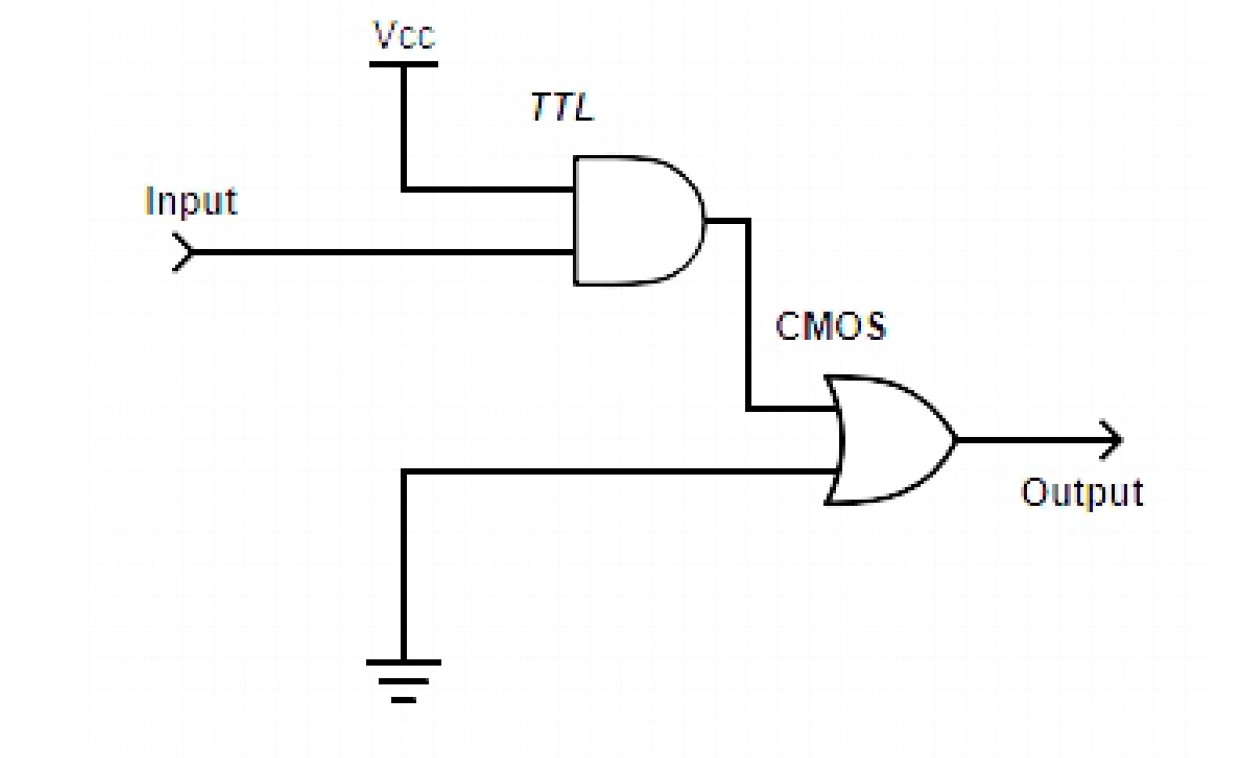
\includegraphics[width=8cm]{ejercicio5/E3_CirEj5.jpg}  
\caption{Circuito ejercicio 5}
\end{figure}


Midiendo en la salida de la OR esperar\'iamos que no hubiera salida o si la hubiera tuviera problemas, ya que la entrada m\'inima que acepta la OR es de 4,2V con la alimentaci\'on elegida y la AND otorga como ya mencionamos 3,5V. En nuestro caso el circuito l\'ogico funcion\'o como si no hubiera ning\'un tipo de problema, creemos que esto puede deberse a que las hojas de datos otorgan datos donde el fabricante se asegura que sus componentes funcionen pero pueden haber algunos que funcionen fuera del alcance determinado por el fabricante, esto quiere decir que puede funcionar pero no esta garantizado el buen funcionamiento. En caso de haber tenido alg\'un error hubi\'eramos optado por utilizar dos transistores para poner un pull-up que se active con la baja salida de la AND y alimente con $V_dd=5V$ la entrada de la OR como en el siguiente esquema.

\begin{figure}[hbtp]
\centering
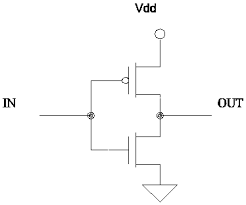
\includegraphics[width=5cm]{ejercicio5/PullUp.jpg} 
\caption{Circuito de Pull-Up}
\end{figure}

